\chapter{Estado del Arte y Marco Tecnológico}

\begin{quotation}[Novelist]{Ernest Hemingway (1899--1961)}
The good parts of a book may be only something a writer is lucky enough to overhear or it may be the wreck of his whole damn life -- and one is as good as the other.
\end{quotation}

\begin{abstract}
En este capítulo presenta el estado del arte y el marco tecnológico que sustenta el desarrollo de \textit{King and Peasant}. En primer lugar, se analizan las soluciones existentes en la digitalización de juegos de mesa, justificando la adopción de un modelo basado en la automatización de reglas frente a la simulación física. A continuación, se detalla y justifica la elección del \textit{stack} tecnológico, abordando la arquitectura de comunicación mediante \textit{WebSockets}, el entorno de ejecución asíncrono en \textit{Node.js}, el renderizado reactivo con \textit{React} y un sistema de persistencia dual basado en \textit{MariaDB} y \textit{Redis}. Finalmente, se expone la estrategia de contenedorización con \textit{Docker} y la política de pruebas automatizadas para garantizar la calidad y portabilidad del sistema.
\end{abstract}

\section{Análisis de soluciones existentes y estado del arte}

En la actualidad existen dos acercamientos a la hora de digitalizar un juego de mesa contemporáneo como lo es \textit{King and Peasant}. Por un lado, tenemos el ejemplo de \textit{Tabletop Simulator} (véase la Figura \ref{fig:tabletop}), que se basa en un entorno de simulación física operando como un "cajón de arena" (\textit{sandbox}) \cite{woods_eurogames}. El cumplimiento de las reglas se delega íntegramente a los usuarios, careciendo de una validación lógica que incrementa la carga cognitiva del usuario y ralentiza el flujo de la partida.

Por otro lado, se encuentra \textit{Board Game Arena} (véase la Figura \ref{fig:bga}), que está basado en un motor de validación de estados. En este modelo el cumplimiento de las reglas y las transiciones de estado se delegan al sistema, actuando así como un árbitro imparcial dentro de la partida garantizando la integridad de las mecánicas \cite{elias_characteristics}. El presente TFG se alinea con este segundo enfoque, ya que lo que se busca es crear un motor de reglas estricto que ofrezca una experiencia de juego automatizada, accesible desde el navegador y libre de la fricción que suponen los simuladores tridimensionales

\begin{figure}[H]
    \centering
    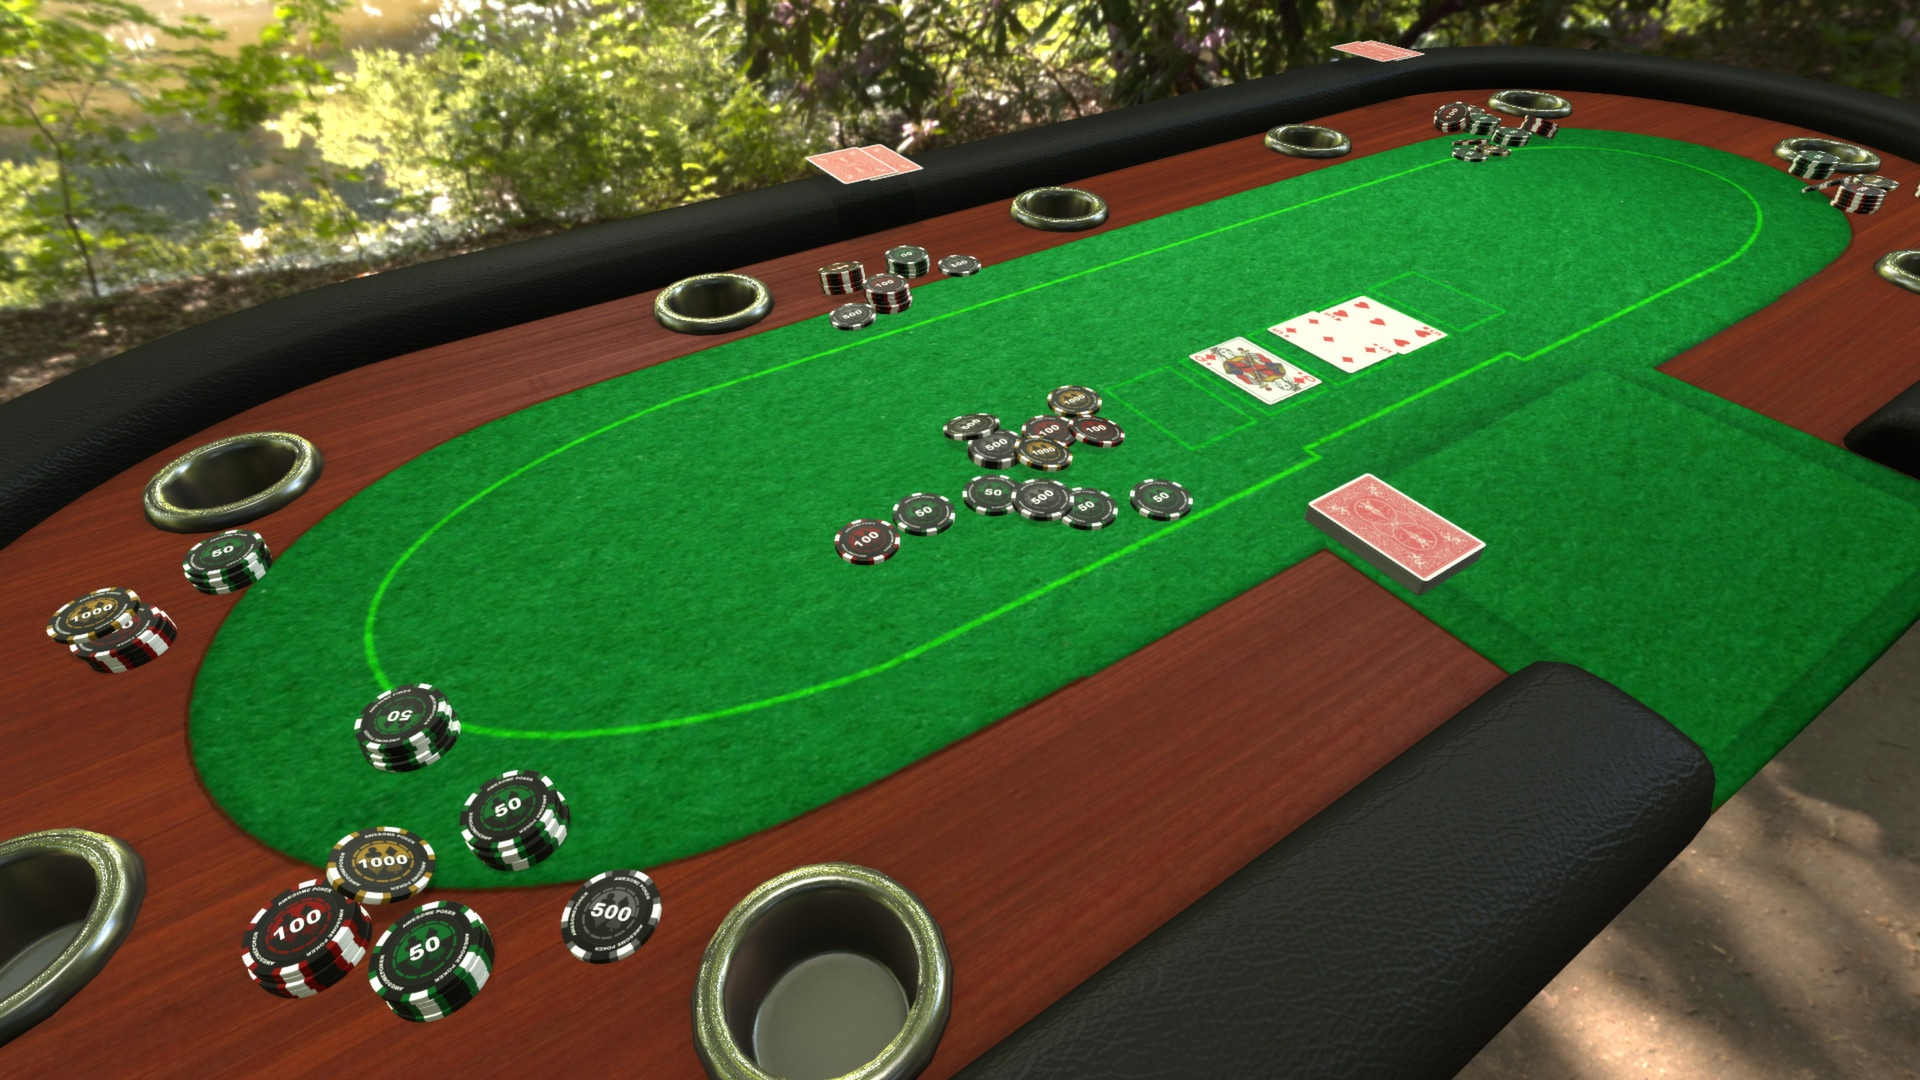
\includegraphics[width=0.8\textwidth]{figures/tabletop-cover_yezh.jpg}
    \caption{Interfaz de \textit{Tabletop Simulator}, basada en la simulación física tridimensional sin validación de reglas.}
    \label{fig:tabletop}
\end{figure}

\begin{figure}[H]
    \centering
    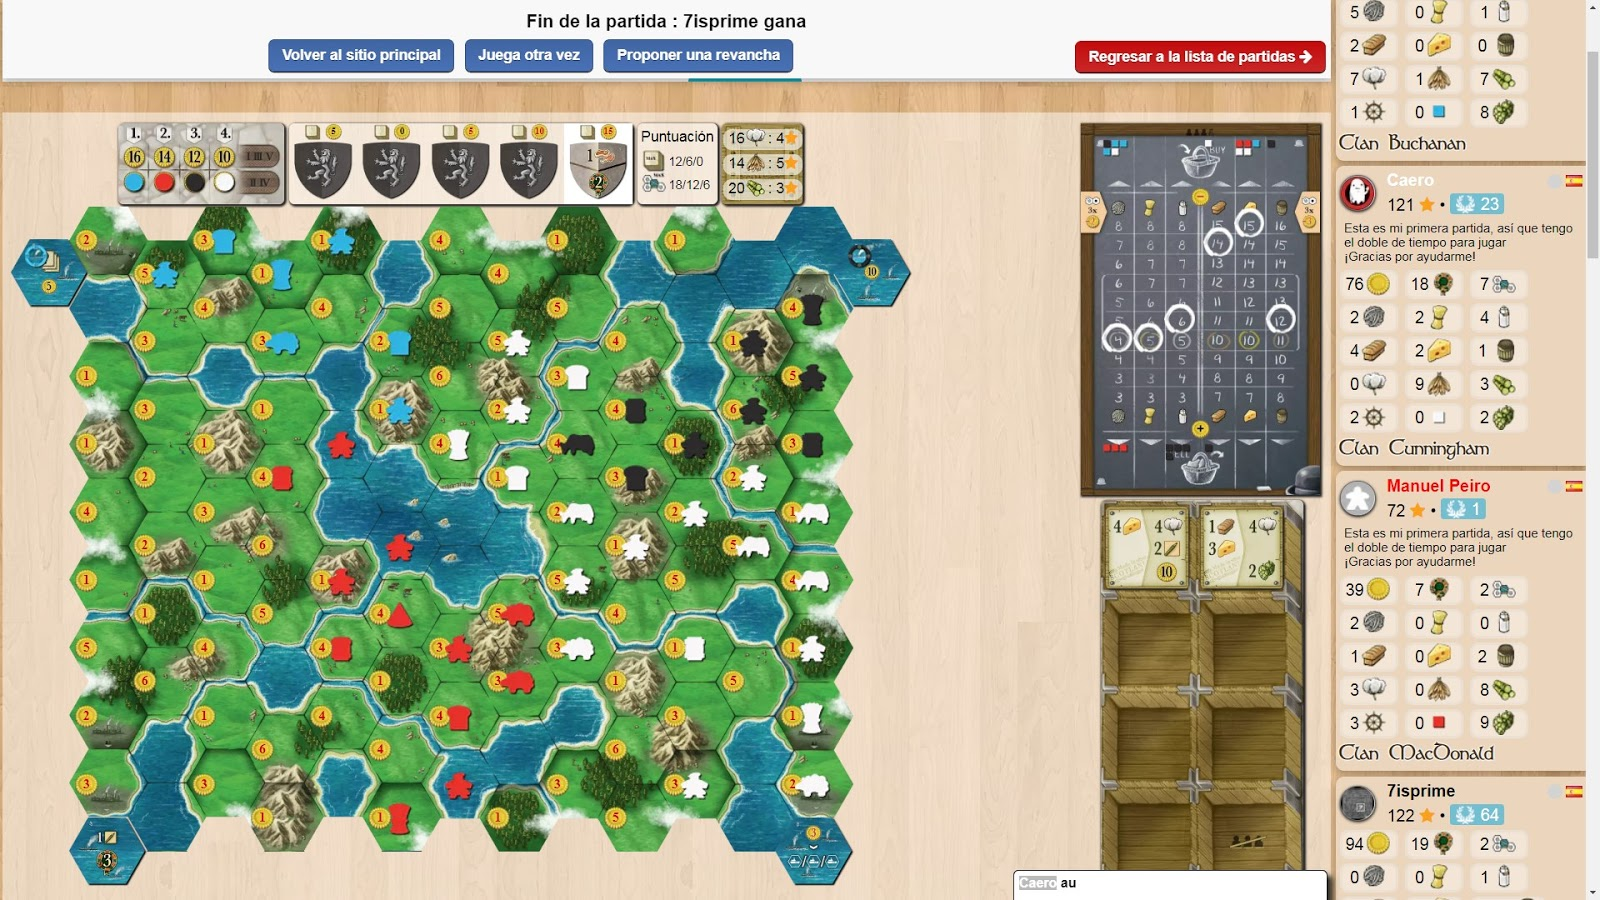
\includegraphics[width=0.8\textwidth]{figures/caledoniaBGALR.jpg}
    \caption{Interfaz de \textit{Board Game Arena}, basada en la automatización del estado de la partida en 2D.}
    \label{fig:bga}
\end{figure}

\section{Arquitectura de comunicación y sincronización}

Dada la naturaleza interactiva de un juego multijugador, la sincronización en tiempo real entre múltiples clientes es un punto crítico dentro del desarrollo de \textit{King and Peasant}. Para este propósito, implementar el motor del juego sobre una arquitectura web tradicional resultaba inviable debido a las limitaciones estructurales del protocolo \textit{HTTP}. El uso de técnicas como el \textit{Long-Polling} (\textit{polling}), donde el cliente interroga constantemente al servidor en busca de actualizaciones, introduciría una sobrecarga significativa en la red debido al envío repetitivo de cabeceras HTTP, generando latencias perceptibles que degradan la experiencia de juego \cite{rfc6202}.

Como alternativa a una API REST, se decidió utilizar el protocolo \textit{WebSocket} como núcleo de las comunicaciones de la partida. Como define el estándar oficial de la IETF \cite{rfc6455}, esta tecnología proporciona un canal de comunicación bidireccional sobre una única conexión TCP persistente. Esto permite el envío de eventos asíncronos (\textit{server-push}) en el mismo instante en el que se modifica el estado, validando las jugadas y actualizando instantáneamente la interfaz de todos los clientes conectados, reduciendo a su vez el coste computacional y garantizando una sincronización  fluida.

\section{Tecnologías de \textit{Backend} y Ecosistema de Desarrollo}

El alto volumen de conexiones concurrentes que presenta un juego multijugador exige un entorno de ejecución capaz de gestionar con eficiencia el consumo elevado de recursos que se produce al mantener las conexiones abiertas en un estado de sincronización permanente. En el caso de los servidores web tradicionales, el modelo de concurrencia basado en hilos (\textit{thread-per-request}) se ve afectado por el cambio de contexto (\textit{context switching}) \cite{tilkov_node}, provocando un rápido agotamiento de la memoria y cuellos de botella. Por otro lado, la mantenibilidad del código y el uso de lenguajes unificados constituyó un factor determinante a la hora de decantarse por una arquitectura de servidor. 

Por estos motivos, se adoptó \textit{Node.js}. Su arquitectura basada en un bucle de eventos (\textit{Event Loop}) procesa las solicitudes de red de forma asíncrona, evitando bloquear el hilo principal durante la espera de respuestas de la base de datos o de los clientes. Este diseño arquitectónico permite al sistema mantener activas miles de conexiones bidireccionales de manera simultánea con un consumo residual de recursos. Además, la capacidad de usar lenguajes isomórficos reduce la sobrecarga cognitiva del equipo de desarrollo y permite la compartición directa de módulos lógicos entre cliente y servidor \cite{cantelon_node}.

\section{Tecnologías de Frontend Reactividad de Interfaz}

La implementación de un juego de mesa en un entorno digital multijugador requiere elementos como un tablero interactivo, el cual, en términos de ingeniería, no es más que la proyección visual de una compleja máquina de estados. Sin embargo, se plantea una serie de retos técnicos a la hora de diseñar este componente. 

En primer lugar, la manipulación directa del \textit{Document Object Model} (DOM) para actualizar la interfaz resulta computacionalmente ineficiente. El navegador se ve obligado a recalcular estilos y repintar la pantalla cada vez que se produce una modificación, lo que provoca que la fluidez de la experiencia se vea degradada \cite{mardan_react}. En segundo lugar, abordar una interfaz que cuenta con tableros, mazos, perfiles y salas de espera bajo una arquitectura monolítica dificultaría enormemente su mantenibilidad y fomentaría la duplicación de código. Finalmente, se le suma el riesgo de desincronización de los estados visuales, resultando en validaciones del \textit{backend} que no se reflejan en la información gráfica \cite{banks_react}.  

Como solución a todos estos problemas, la arquitectura del cliente se construyó utilizando \textit{React}, una librería que impone un paradigma de desarrollo declarativo y basado en componentes. En primer lugar, gracias a la implementación de un \textit{Virtual DOM}, la ineficiencia computacional se mitiga. Al recibir un nuevo evento, \textit{React} genera una representación en memoria de la interfaz y la compara con la actual mediante un algoritmo de diferenciación (\textit{diffing}), aplicando al DOM real únicamente las modificaciones estrictamente necesarias. En segundo lugar, su arquitectura modular minimiza el riesgo que supone construir un sistema monolítico, permitiendo dividir la interfaz en unidades lógicas aisladas e independientes, facilitando la encapsulación y garantizando la mantenibilidad a largo plazo del código. Por último, el paradigma declarativo de \textit{React} permite concibir la interfaz matemáticamente como una función del estado subyacente ($UI = f(estado)$) \cite{banks_react}, convirtiendo el tablero en un reflejo exacto de la información de la partida y las reglas dictaminadas por el \textit{backend} \cite{mardan_react}.

\section{Gestión de la persistencia de datos}

Dentro de la información gestionada por el ecosistema encontramos requisitos técnicos independientes, lo que implica la necesidad de implementar un enfoque de persistencia adecuado para cada uno de ellos fundamentado en su naturaleza. Por un lado, la información estructural, como pueden ser las credenciales, perfiles de usuario, historial de partidas o la gestión de salas de espera (\textit{lobbies}), exige un almacenamiento persistente y estructurado que garantice las propiedades ACID (Atomicidad, Consistencia, Aislamiento y Durabilidad) \cite{elmasri_db}. Para satisfacer esta necesidad, y tras evaluar alternativas relacionales robustas como \textit{PostgreSQL}, se seleccionó el motor de bases de datos relacional \textit{MariaDB} por su agilidad en consultas y su perfecta integración con el ecosistema de \textit{Node.js}. Este motor se encarga de gestionar de forma centralizada la información de los usuarios y la configuración inicial de las partidas. La interacción con este motor relacional se abstrajo mediante \textit{Prisma ORM}, una decisión que previene vulnerabilidades de inyección SQL y garantiza un tipado estricto entre el esquema de la base de datos y la lógica del \textit{backend}.

Por otro lado, el estado del tablero interactivo se convierte en un dato efímero sometido a un volumen masivo de operaciones de lectura y escritura concurrentes. Hacer uso de una base de datos relacional para registrar las modificaciones generaría un cuello de botella debido a la latencia de entrada/salida (I/O), ralentizando la comunicación. Para mitigar este problema, se implementó \textit{Redis} como almacén de estructuras de datos en memoria (\textit{In-Memory Data Grid}) \cite{carlson_redis}. A diferencia de sistemas de caché simples como \textit{Memcached}, \textit{Redis} soporta el manejo nativo de estructuras de datos complejas, una característica indispensable para modelar el estado de un juego. Hacer uso de la memoria RAM para almacenar el estado dinámico de la partida permite que el servidor valide y comparta el resultado de las jugadas con tiempos de respuesta mucho menores, delegando en \textit{MariaDB} la persistencia del resultado final una vez concluido el encuentro.

\section{Contenedorización y automatización de pruebas}

El complejo funcionamiento intrínsico del motor de reglas asimétrico requería mecanismos rigurosos para garantizar la calidad y la estabilidad del software. El mal funcionamiento de las validaciones de estado o de las transiciones de la partida degradaría la experiencia de juego. En respuesta, haciendo uso de los marcos de trabajo \textit{Jest} y \textit{Vitest}, se implementó una batería de pruebas automatizadas que aseguraban el correcto comportamiento del motor de validación ante cualquier escenario \cite{myers_testing}. Dichas herramientas han permitido aislar y testear unitariamente la lógica del \textit{backend} y los componentes del \textit{frontend}.

De forma paralela, la gestión de la infraestructura se apoyó en la tecnología de contenedores \textit{Docker} \cite{turnbull_docker}. El principal problema que se buscó mitigar con esta adopción fue la inconsistencia de entornos al tratarse de un desarrollo colaborativo entre dos personas. Resultaba necesario aislar los servicios para evitar fallos derivados de las diferencias de \textit{hardware} o configuración del sistema operativo. Por este motivo, se estableció una arquitectura de ejecución híbrida. Por un lado, los servicios de bases de datos (\textit{MariaDB} y \textit{Redis}) se ejecutan exclusivamente mediante contenedores, garantizando que el equipo opere siempre sobre versiones idénticas de estos sistemas. Por otro lado, la capa de aplicación (\textit{frontend} y \textit{backend}) se implementó con un modelo flexible que permite su lanzamiento en local para agilizar la iteración de código, o bien su ejecución contenedorizada. A su vez, esta estandarización de los servicios resulta idónea para simplificar y asegurar el futuro despliegue de la plataforma en entornos de producción.